% ============================================================
%  §3 增强导出范畴 / §4 Fukaya 范畴（原文 pp.13–21）
%  原文：3. The enhanced derived category；4. The Fukaya category
%        （含 4.1、4.2、4.2.1、4.3、4.3.1、4.3.2、4.4）
%  说明：p.13 顶端 "Proof. By the lemma, …" 属 §2 末尾，不在本文件。
%        原文编号公式 (2) 见 eq:derived-1；图 1 见 fig:dehn-twist。
% ============================================================

\section{增强导出范畴}
\label{sec:derived}

% [Tutor Note: 本节的 "dg-范畴" 指 Hom 空间是 $\mathbb{Z}$-分次复形、复合满足 Leibniz 法则的范畴。关键是把 $\Hom$ 从向量空间升级为复形：$\Hom^\bullet(I_A,I_B)$ 的微分来自 $I_A,I_B$ 各自的内部微分，取上同调才得到 $\Ext$。这就是 "enhanced" 的含义——普通导出范畴只记住 $H^0$，会丢失 $m_1$ 以上的高阶信息（$A_\infty$ 结构）；而在同调镜像对称中，$A_\infty$ 运算恰恰是必须逐项比较的数据，故必须在这一层做 dg-增强。]

\begin{keytakeaways}
  \item \textbf{物理/几何图像}：概形上凝聚层的导出范畴是 B-模型 D-膜（B-brane）的数学载体；用内射消解把 Hom 空间提升为复形（dg-增强）后，它才成为可与 A-模型（Fukaya 范畴）逐对象、逐态射比较的 $A_\infty$-范畴。
  \item \textbf{数学工具}：内射消解 + Hom 复形；$\Ext$ 与 $H^*\Hom^\bullet$ 的等同由一个弱收敛谱序列给出（命题 \ref{prop:3.1}）。
  \item \textbf{核心结论}：$\Dinf(X)$ 分裂闭且三角；光滑射影簇上由局部自由层生成，更强地由线丛 $\cO_X(n)$（$n\in\ZZ$）分裂生成；代数曲线上只需 $\cO_X$ 与 $\cO_X(P)$ 即可分裂生成——这给出 HMS 一侧所需的最小生成元清单。
\end{keytakeaways}

我们现在构造第一个真正有趣的 $A_\infty$-范畴：概形上凝聚层的导出范畴。关于阿贝尔范畴与同调代数的基础参考见 [23]；概形理论的一般参考见 [8]。

设 $\cB$ 是含足够多内射对象的阿贝尔范畴，$\cA\subset\cB$ 是全子范畴。则对 $\cA$ 中每个有界复形 $A^\bullet$，在 $\cB$ 中存在与它拟同构的左有界内射复形 $I_A^\bullet$（例如 Cartan–Eilenberg 消解，见 [23, 第 5.7 节]）。由标准论证，任意两个这样的复形彼此拟同构，且在链同伦意义下唯一。

% [Tutor Note: "任意两个这样的复形互相拟同构，且在链同伦意义下唯一" 即内射消解的比较定理；"唯一到同伦" 比通常的 "唯一到拟同构" 强，依据是内射对象关于消解映射的提升性质，再逐级归纳（左有界性保证每一步只涉及有限次延拓）。若把 $\mathcal B$ 换成一般加性范畴，这两条都会失效——这正是命题 3.1 要求 $\mathcal B$ 有足够多内射对象的原因。]

设已为每个有界复形 $A$ 选定这样的 $I_A$。我们把 $\cA$ 的（相对于 $\cB$ 的）\emph{增强导出范畴}（enhanced derived category）记作 $\Dinf(\cA,\cB)$。定义 $\Ob(\Dinf(\cA,\cB))$ 由 $\cA$ 中的有界复形组成，并令
\[
  \Hom_{\Dinf(\cA,\cB)}(A^\bullet, B^\bullet) = \Hom^\bullet(I_A, I_B).
\]
这自然地是一个 dg-范畴。

% [Tutor Note: 注意 $\Hom^\bullet(I_A,I_B)$ 的微分有两种来源（$I_A$ 的内部微分与 $I_B$ 的内部微分，带 Koszul 符号），复合 $f\mapsto g\circ f$ 满足分次 Leibniz 法则；这是 "dg-范畴" 而非仅仅 "分次范畴" 的全部内容。此外 $I_A$ 只是 $A$ 的消解，故 $\Hom_{\Dinf}(A^\bullet,B^\bullet)$ 不依赖 $A^\bullet$ 的特定代表，依赖的是消解的选取——命题 \ref{prop:3.1} 说明这一依赖在同伦意义下消失。]

\begin{proposition}\label{prop:3.1}
dg-范畴 $\Dinf(\cA,\cB)$ 与消解复形 $I_A$ 的选取无关，在拟同构意义下唯一。此外
\[
  H^*\Hom_{\Dinf(\cA,\cB)}(A,B) \simeq \Ext^*(A,B).
\]
\end{proposition}

\begin{proof}
设 $I'_A$ 是另一组消解。由内射对象的一般结果，$A$ 上的恒等态射可提升为一对互逆的拟同构 $\alpha_A: I_A\to I'_A$ 与 $\beta_A: I'_A\to I_A$。可以验证，态射
\[
  f_A = (\alpha_A^*, \beta_{B*}) : \Hom^\bullet(I_A, I_B) \to \Hom^\bullet(I'_A, I'_B)
\]
定义了两个范畴之间一个 dg-函子的 $F_1$ 项（该函子在对象上是恒等）。$F_2$ 项由 $\beta_A\alpha_A$ 与 $\mathbf 1$ 之间的同伦组成。

% [Tutor Note: $f_A=(\alpha_A^*,\beta_{B*})$ 的记号是 "前复合 $\alpha_A$、后复合 $\beta_B$"，即 $\varphi\mapsto \beta_B\circ\varphi\circ\alpha_A$；原文把 $\alpha_A$ 的上标与 $\beta_B$ 的下标写得并不对称，容易误读成两种不同的函子性。核对时可直接按 "$\alpha$ 前复合、$\beta$ 后复合" 理解。]

于是只需证明 $f_A$ 是拟同构。为此可用弱收敛谱序列
\[
  E_1^{p,q} = H^p\Hom_{\cA}(C^{-\bullet}, I_B^q) \Rightarrow H^{p+q}\Hom^\bullet(C, I_B).
\]
拟同构 $C\to C'$ 在 $E_1$ 页上诱导同构，因而在上同调中诱导同构。把它应用于 $A\to I_A$，即得 $H^*\Hom^\bullet(I_A,I_B)\simeq\Ext^*(A,B)$。故 $f_A$ 是拟同构。
\end{proof}

% [Tutor Note: 该谱序列来自双复形 $\Hom(C^{-\bullet}, I_B^\bullet)$：$p$ 是 $C$ 的次数、$q$ 是 $I_B$ 的次数。"weakly convergent"（弱收敛）是必要的，因为 $C$ 只单侧有界，$E_1$ 页可能出现无限多列；逐列有限才保证收敛。另外原式的 $C^{-\bullet}$ 带一个上标负号，文中从未定义此记号，疑为 $C^\bullet$ 的笔误或某种截断约定，阅读时先按 $C^\bullet$ 理解不影响论证。]

% [Tutor Note: $F_2$ 项是 $\beta_A\alpha_A$ 与 $\mathbf 1$ 之间的同伦族，这就是 $A_\infty$-函子比 dg-函子多出来的部分：因为 $\beta_A\alpha_A$ 只在同伦意义下是恒等，$f_A$ 严格说来不是 dg-函子而是 $A_\infty$-函子（$F_{\ge 3}=0$）。把 "拟同构" 升级为 "拟等价" 时，正是靠这个 $F_2$ 取逆。]

\begin{definition*}
设 $X$ 是代数簇（域上有限型概形）。则 $X$ 的\emph{增强导出范畴}记作 $\Dinf(X)$，它是 dg-范畴 $\Dinf(\Coh(X), \mathrm{QCoh}(X))$，在拟同构意义下良定义。
\end{definition*}

% [Tutor Note: 原文的这个 Definition 不带编号（故用 definition* 环境），命题 3.1 与定理 3.2 的编号因此与原文一致。]

这里 $\Coh(X)$ 表示凝聚层范畴，$\mathrm{QCoh}(X)$ 表示拟凝聚层范畴。

可以证明 $\Dinf(X)$ 事实上是分裂闭的且是三角范畴。三角结构本质上是显然的；分裂闭性例如在 [19, 第 (5c) 节] 中有证明。我们其实并不需要这些结果，但它意味着我们不必书写（也不必考虑）$D^\pi\Dinf(X)$。

% [Tutor Note: $D^\pi$ 是 §2 中定义的分裂闭三角包络（split-closed triangulated envelope）。作者说 "不必写 $D^\pi\Dinf(X)$" 的意思是：$\Dinf(X)$ 自身已经是分裂闭的三角 $A_\infty$-范畴，故 $D^\pi\Dinf(X)$ 与 $\Dinf(X)$ 拟等价，取包络是多余的。"三角结构显然" 的实质是：映射锥可在 dg 层直接写出，且 dg 层的锥与同伦范畴中的锥一致；对一般的 $(\mathcal A,\mathcal B)$ 则未必。]

事实上可以证明，$H^0\Dinf(X)$ 就是由 $D^b(\Coh(X))$ 反转拟同构所得的范畴（这一点对上述一般的二元组 $(\cA,\cB)$ 并不成立），但我们并不需要它。下面证明增强导出范畴的两个生成结果。

% [Tutor Note: 此句是全文少数几个 "只对 $(\Coh,\mathrm{QCoh})$ 成立" 的陈述之一：把 $\mathcal A$ 中对象换成 $\mathcal B$ 中的消解后，$H^0$ 一般只是某个局部化，未必等于 $D^b(\mathcal A)$。原文特意加括号提醒，读者不要把它当成对任意 $(\mathcal A,\mathcal B)$ 的定理。]

\begin{theorem}\label{thm:3.2}
设 $X$ 是带极丰沛线丛 $\cO(1)$ 的光滑射影簇。则 $\Dinf(X)$（作为三角 $A_\infty$-范畴）由局部自由层生成。此外，$\Dinf(X)$ 由线丛 $\cO_X(n)$（$n\in\ZZ$）分裂生成。
\end{theorem}

\begin{proof}
$\Dinf(X)$ 由 $\Coh(X)$ 生成是清楚的。我们首先证明每个凝聚层都有自由消解。由射影概形上拟凝聚层的分类，每个凝聚层 $\cF$ 对充分大的 $n$ 与 $m$ 都存在满射 $\cO(-n)^m\to\cF$。固定 $\cF\in\Coh(X)$，可构造消解
\begin{equation}\label{eq:derived-1}
  0 \to \mathcal{R} \to \cO(-n_l)^{m_l} \to \cdots \to \cO(-n_1)^{m_1} \to \cF \to 0 .
\end{equation}
现在回忆层 $\Ext$ 函子（见 [8, III.6]）。由标准的（维数平移）论证，$\Ext^i(\mathcal{R},\mathcal{G}) = \Ext^{i+l}(\cF,\mathcal{G})$。我们断言：对任意 $\mathcal{G}\in\mathrm{QCoh}(X)$ 与 $i>\dim X$，它为零。事实上，只需逐茎证明，而
\[
  \Ext^i(\cF,\mathcal{G})_x = \Ext^i_{\cO_{X,x}}(\cF_x,\mathcal{G}_x) = 0
  \qquad (i > \dim X \ge \operatorname{cd}\cO_{X,x}),
\]
这由 Serre 关于正则局部环上同调维数的定理给出。由此可知，若 $l>\dim X$，则对任意 $x\in X$，$\mathcal{R}_x$ 是自由模（因为 Noether 局部环上有限生成投射模自由），从而 $\mathcal{R}$ 是局部自由层（因为 $X$ 是 Noether 的）。第一个断言得证。

% [Tutor Note: 维数平移中的 $l$ 就是消解 \eqref{eq:derived-1} 里 $\cO(n)$ 项的个数；注意 $\Ext^i(\mathcal R,\mathcal G)=\Ext^{i+l}(\cF,\mathcal G)$ 的下标是相加，写成相减是本段最常见的错误。逐茎等式 $\Ext^i(\cF,\mathcal G)_x=\Ext^i_{\mathcal O_{X,x}}(\cF_x,\mathcal G_x)$ 用的是 $\Ext$ 层与局部化交换，属凝聚层理论的标准事实；"$\dim X\ge\operatorname{cd}\cO_{X,x}$" 中 cd 指上同调维数，正则局部环的 cd 等于其 Krull 维数。]

对第二个断言，注意正合列 \eqref{eq:derived-1} 在 $\Dinf(X)$ 中给出正合三角形
\[
  \mathcal{R}[l-1] \to \mathcal{L}^\bullet \to \cF \to ,
\]
其中 $\mathcal{L}^\bullet$ 表示由各 $\cO(n)$ 拼成的复形。旋转三角形，得到正合三角形 $\cF \to \mathcal{R}[l] \to \mathcal{L}^\bullet[1] \to$。然而由命题 \ref{prop:3.1}，$\Hom_{H^0\Dinf(X)}(\cF,\mathcal{R}[l]) = \Ext^l(\cF,\mathcal{R})$。我们断言当 $l$ 充分大时它也为零。若如此，则 $\mathcal{L}^\bullet[1]$ 拟同构于零态射 $\cF\to\mathcal{R}[l]$ 上的锥，而该锥正是直和 $\cF\oplus\mathcal{R}[l]$，定理得证。

% [Tutor Note: 三角形 $\mathcal R[l-1]\to\mathcal L^\bullet\to\cF\to$ 的平移指标很容易错。按原文约定（$[n]$ 表示次数加 $n$）：把 $\cF$ 放在次数 $0$、$\cR$ 放在次数 $-l$，则 $\mathcal L^\bullet$ 占据次数 $-l,\dots,-1$，此时 $\mathcal R[l-1]$ 的支撑次数为 $-1$，恰好接上 $\mathcal L^\bullet$ 的末项——这才是 $[l-1]$ 而不是 $[l]$ 的来源。旋转三角形时 $[l-1][1]=[l]$ 给出第二个三角形。]

为证明该断言，利用 Ext-到-Ext 谱序列可以看出：若 $\Ext^i(\cF,\mathcal{G})=0$ 对 $i>n$ 成立，则 $\Ext^i(\cF,\mathcal{G})=0$ 对 $i>n+\dim X$ 成立（因为对任意拟凝聚层 $\mathcal{G}$ 有 $H^p(X,\mathcal{G})=0$，$p>\dim X$）。而这在上面已经证明过（取 $n=\dim X$）。
\end{proof}

% [Tutor Note: 这段里同一个记号 $\Ext$ 指两个不同对象，是全节最易漏读之处：前提中的 "$\Ext^i(\cF,\mathcal G)=0$（$i>n$）" 说的是层 $\Ext$（即 $\mathcal Ext$，逐茎给出）；结论中的才是整体 $\Ext$。桥接二者的正是 Ext-到-Ext 谱序列 $H^p(X,\mathcal Ext^q(\cF,\mathcal G))\Rightarrow\Ext^{p+q}(\cF,\mathcal G)$：层 $\Ext^q$ 在 $q>n$ 时为零，而 $H^p(X,-)$ 在 $p>\dim X$ 时为零，两者相加就得到 $i>n+\dim X$ 的整体消失。原文用同一符号书写，须自行区分。]

% [Tutor Note: "当 $l$ 充分大时 $\Ext^l(\cF,\mathcal R)=0$" 保证了 $\cF\to\mathcal R[l]$ 是同伦意义下的零态射，因此其锥分裂为直和——这是 "split-generated" 中 "split" 一词的实际来源：不是直接构造直和分解，而是通过消去一个零态射的锥得到直和项。]

\begin{theorem}\label{thm:3.3}
设 $X$ 是代数闭域上的代数曲线（一维光滑射影簇），$P\in X$ 是闭点。则 $\Dinf(X)$ 由 $\cO_X$ 与 $\cO_X(P)$ 分裂生成。
\end{theorem}

\begin{proof}
由 Riemann–Roch 定理与嵌入判别法（[8, remark II.7.8.2]），$\cO(P)$ 是丰沛的。因此只需证明由 $\cO$ 与 $\cO(P)$ 分裂生成的范畴 $\cC$ 包含 $\cO(nP)$，$n\in\ZZ$。但我们有正合列
\[
  0 \to \cO(nP) \to \cO((n+1)P) \to \cO/P \to 0 .
\]
$n=0$ 的情形说明 $\cO/P\in\cC$。于是对 $n$ 归纳即知 $\cO(nP)\in\cC$ 对任意 $n$ 成立。
\end{proof}

% [Tutor Note: 原文写 $\cO/P$，应理解为 $\cO_X/\cO_X(-P)$，即支撑在 $P$ 处的摩天层；正合列中的第三个映射就是 "在 $P$ 处取值"。另外 "对任意 $n\in\mathbb Z$" 包含负 $n$，正向归纳只覆盖 $n\ge 0$；对负 $n$ 要把同一正合列反向使用（$\cO(nP)$ 是 $\cO((n+1)P)\to\cO/P$ 的核），而分裂闭三角范畴对锥、从而对核封闭，故结论仍成立。原文 "induction on $n$" 未说明这一点。]

\section{Fukaya 范畴}
\label{sec:fukaya}

% [Tutor Note: 本节只写 "环面 + 选定 Maslov 覆盖" 的情形，这是全文唯一真正落地的 A-模型。一般辛流形的 Fukaya 范畴需要处理伪全纯圆盘的紧性、Kuranishi 结构、多纤维的横截性等，作者明言 "不给出全部细节"。阅读时应把每个定义都先按 $T=\mathbb C/\mathbb Z^2$ 来理解，再考虑哪些论证对高维成立。]

\begin{keytakeaways}
  \item \textbf{物理/几何图像}：Fukaya 范畴的对象是带分次的拉格朗日 D-膜，态射空间由横截交点张成；$A_\infty$ 运算 $m_n$ 数的是边界落在给定拉格朗日上的全纯（伪全纯）多边形，其权重是 $t^{\int u^*\omega}$，即多边形面积。
  \item \textbf{数学工具}：Maslov 指标与 Maslov 类（关键在于 $\mathrm{LGr}(V)$ 的 $\pi_1=\ZZ$）；$\ZZ$-分次的 Maslov 覆盖；局部模型 + Weinstein 邻域移植得到的 Dehn 扭转。
  \item \textbf{核心结论}：\emph{Fukaya 范畴} $\Fuk(T)$ 的对象是分次拉格朗日圆周；$\Sym^{gr}(T)$ 作用于 $\Fuk(T)$，且哈密顿同伦于恒等的分次辛同胚作用拟同构于恒等函子；代数扭变函子 $T_L$ 与辛 Dehn 扭转 $\tilde\tau_L$ 在对象上一致（定理 \ref{thm:4.2}）。
\end{keytakeaways}

本节勾画 Fukaya 范畴（Fukaya category）的构造。一般情形下这非常困难，我们无法给出全部细节。我们将侧重那些能推广到高维的材料，而对只适用于环面的细节则压缩到最低限度。更完整的叙述见 [19, 第 8、9 节] 与 [20]。

前两个小节回顾辛几何的一些基本概念。概览性的介绍例如见 [4]。

\subsection{辛线性空间}
\label{subsec:sympl-linear}

回忆：\emph{辛向量空间}（symplectic vector space）是有限维实向量空间 $V$，连同一个非退化反对称双线性形式 $\omega$。\emph{相容复结构}是自同构 $I: V\to V$，满足 $I^2=-1$，且 $g(v,w)=\omega(v,Iw)$ 是正定（双线性对称）形式。相容的 Riemann 内积类似地定义。这样得到的三元组 $(\omega,I,g)$ 称为\emph{相容的}；容易看出相容三元组总是存在。若 $(\omega,I,g)$ 是相容三元组，则 $h=g+I\omega$ 在 $V$（视为复向量空间）上定义 Hermite 内积。

% [Tutor Note: 原文写 $h=g+I\omega$，其中 $I$ 作用在第二个变量上，展开即 $h(v,w)=g(v,w)+i\,\omega(v,w)$（$\omega$ 反对称、$g$ 对称，故 $h$ 是 Hermite 的）。这里 $\omega$ 与 $g$ 定义在同一实空间上，$I\omega$ 是复合而非复数 $i$ 乘 $\omega$；若把 $I$ 作用在第一个变量上，得到的是复共轭，两种约定只差一个复共轭，但会改变 $s(L)$ 的相位，核对符号时要注意。]

众所周知，辛向量空间必为偶数维 $2n$。子空间 $L\subset V$ 称为\emph{拉格朗日的}（Lagrangian），若 $\dim L=n$ 且 $\omega|_L=0$，即对所有 $v,w\in L$ 有 $\omega(v,w)=0$。回忆存在以 $V$ 的 $m$ 维子空间为点的拓扑空间 $\mathrm{Gr}(m,V)$。我们用 $\mathrm{LGr}(V)\subset\mathrm{Gr}(n,V)$ 记 $V$ 的所有拉格朗日子空间构成的\emph{拉格朗日 Grassmann 流形}（Lagrangian Grassmannian）。

选取相容三元组 $(\omega,I,g)$，即得 $V$ 上的 Hermite 内积。于是容易看出，每个拉格朗日子空间都等于 $V$（作为复向量空间）的某组 Hermite 基的实张成。因此
\[
  \mathrm{LGr}(V) \simeq U(n)/O(n).
\]
由此可知 $\mathrm{LGr}(V)$ 连通（因为 $U(n)$ 连通），且基本群为 $\ZZ$（考虑显然的纤维化）。

% [Tutor Note: "consider the evident fibration" 指 $\mathrm{LGr}(V)\cong U(n)/O(n)$ 上的行列式平方映射 $\det^2: U(n)/O(n)\to S^1$，其纤维为 $SU(n)/SO(n)$（$n\ge 1$ 时单连通），故 $\pi_1(\mathrm{LGr}(V))\cong\pi_1(S^1)=\ZZ$。这一点是全局的关键：$\pi_1=\ZZ$ 才使万有覆盖存在，$\ZZ$-作用才给出分次平移 $[n]$，Floer 复形才是 $\ZZ$-分次的而不是仅 $\ZZ/2$-分次的。]

固定相容三元组 $(\omega,I,g)$，记 $h$ 为相应的 Hermite 度量。用 $\Lambda^n_{\CC}V$ 记 $V$（作为复向量空间）的最高外幂。这是一条复直线，其上带有 Hermite 度量。对由 Hermite 基 $e_1,\dots,e_n$ 张成的拉格朗日子空间 $L=\langle e_1,\dots,e_n\rangle$，令
\[
  s(L) = \frac{(e_1\wedge\cdots\wedge e_n)^{\otimes 2}}
               {|e_1\wedge\cdots\wedge e_n|^2} .
\]
这是良定义的映射 $\mathrm{LGr}(V)\to S(\Lambda^n_{\CC}V^{\otimes 2})$，其中右端表示一条复直线的单位圆。它因而带有自然的定向，从而带有 $H^1$ 的一个生成元。用 $s$ 拉回这个生成元，得到元素 $s_V\in H^1(\mathrm{LGr}(V),\ZZ)$，称为 \emph{Maslov 类}（Maslov class）。可以证明它事实上是 $H^1(\mathrm{LGr}(V),\ZZ)$ 的一个生成元，且只依赖 $\omega$，不依赖 $I$ 与 $g$。于是若 $\gamma$ 是 $\mathrm{LGr}(V)$ 中的环路，可写 $[\gamma]=n s_V$，从而得到整数 $n$。

% [Tutor Note: 公式里的平方不是装饰：拉格朗日子空间没有定向，Hermite 基的选取只确定到 $O(n)$ 的元素，于是 $\det(e_1,\dots,e_n)$ 只能确定到符号 $\pm1$；取 $(\cdot)^{\otimes 2}$ 恰好消去这个符号，$s$ 才良定义。分母的模长平方把它归一到单位圆。若改用行列式本身（不平方），得到的将是 "Maslov 类的平方根"，会出现符号反常——这正是 A-模型在一般情形需要 spin/Pin 结构的技术根源。]

所谓的 \emph{Maslov 指标}（Maslov index）是对这一观察的宏大推广。

\begin{theorem}\label{thm:4.1}
固定 $V$ 的两个拉格朗日子空间 $L_1$ 与 $L_2$，并用 $P(V,L_1,L_2)$ 记道路 $\gamma:[0,1]\to\mathrm{LGr}(V)$（满足 $\gamma(0)=L_1$、$\gamma(1)=L_2$）构成的空间。其上带有自然的等价关系 $\gamma_1\sim\gamma_2$，由相对于 $\{0,1\}$ 的同伦给出。

可以定义一族函数 $\mu: P(V,L_1,L_2)\to\ZZ$，具有如下性质：(1) $\mu$ 通过 $\sim$ 分解；(2) 当 $L_1=L_2$ 时 $\mu$ 化为上面定义的环路 Maslov 指标；(3) $\mu$ 只依赖 $V$ 的辛结构，不依赖任何其他选择。

现在设 $\dim V=2$。取保定向的同胚 $S(\Lambda^n_{\CC}V)^{\otimes 2}\simeq S^1$。则对环路 $\gamma:[0,1]\to\mathrm{LGr}(V)$，有
\[
  \mu(\gamma) = [f(1)],
\]
其中 $f$ 表示 $s\gamma$ 到 $\RR$ 的唯一提升，满足 $f(0)=0$，相对于覆盖 $\RR\to S^1$，$x\mapsto e^{2\pi i x}$；而 $[x]$ 表示不大于 $x$ 的最大整数。
\end{theorem}

% [Tutor Note: 定理只列了三条性质，确实不足以唯一确定 $\mu$（在每条同伦类上还可加一个只依赖 $(L_1,L_2)$ 的常数），作者自己也说 "只作示意"。真正被这三条钉住的是 "差"：$\mu(L_1,L_2)+\mu(L_2,L_3)=\mu(L_1,L_3)$；而 (2) 把环路情形归到 $s_V$ 的度上。]

% [Tutor Note: 原文疑误（或冗余）：$\gamma$ 是环路，故 $s\gamma$ 是 $S^1$ 中的环路，$f(1)\in\mathbb Z$ 自动成立，$[\cdot]$ 的取整在此是多余的。取整只在讨论 "道路"（两端点不闭合）时才有意义。另注意第二条中应读作 $s\circ\gamma$，且 $\dim V=2$ 时才有 $S(\Lambda^n_{\mathbb C}V)\cong S^1$ 这种可写的同胚。]

% [Tutor Note: 原文疑误：这里的目标空间写成 $S(\Lambda^n_{\mathbb C}V)^{\otimes 2}$，而本节前面 $s$ 的像定义为 $S(\Lambda^n_{\mathbb C}V^{\otimes 2})$；两者是同一个对象的不同写法吗？不是——单位圆上的平方映射 $z\mapsto z^2$ 并不等同。按前文自洽的写法，此处应为 $S(\Lambda^n_{\mathbb C}V^{\otimes 2})\simeq S^1$。译文保留原文。]

定理中描述的性质并不决定 $\mu$，这些性质只作示意。第一部分在 [2] 中得到证明；那里还公理化地刻画了 Maslov 指标，并以多种方式构造了它。定理的第二部分在 Maslov 指标定义好之后是一个容易的练习。

\subsection{一些辛几何}
\label{subsec:sympl-geom}

回忆：\emph{辛流形}（symplectic manifold）是光滑实流形 $M$，连同一个闭的、非退化的二形式 $\omega=\omega_M$。于是对每点 $x\in M$，$M$ 在 $x$ 处的切空间 $T_xM$ 自然地是辛向量空间。辛流形 $(M,\omega)$ 与 $(N,\eta)$ 之间的\emph{辛同胚}（symplectomorphism）是光滑映射 $f: M\to N$ 且 $f^*\eta=\omega$。$M$ 的辛自同构群记作 $\Sym(M)=\Sym(M,\omega)$。

如前，辛流形必为偶数维 $2n$。$n$ 维子流形 $L\subset M$ 称为\emph{拉格朗日的}，若 $\omega|_L=0$。等价地，对每个 $x\in L$，$T_xL\subset T_xM$ 是拉格朗日子空间。若 $\phi: M\to M$ 是辛自同构，则 $\phi(L)$ 也是拉格朗日子流形。

现设 $X_t$ 是 $M$ 上（可随时间变化的）向量场，且 $M$ 紧。回忆此时存在唯一流 $\phi_t: M\to M$ 使 $\partial\phi/\partial t=X_t$。若 $\phi_t$ 是辛同胚，则称 $X_t$ 为\emph{辛向量场}。这成立当且仅当一次形式 $\eta_{X_t}(v):=\omega(X_t,v)$ 闭（这由 Cartan 公式得出）。此时称族 $\phi_t$ 为\emph{辛同伦}（isotopy，从 $\phi_0=\mathbf 1$ 到 $\phi_1$）。若 $\eta_X$ 不仅闭而且恰当，比如 $\eta_{X_t}=dH_t$，则称 $\phi_t$ 为对应于 \emph{哈密顿函数} $H$ 的\emph{哈密顿同伦}。注意 $\omega$ 的非退化性蕴涵：对每个一次形式 $\eta$ 恰有一个向量场 $X$ 使 $\eta_X=\eta$。因此对每个（可随时间变化的）哈密顿函数 $M\times[0,1]\to\RR$，我们都得到一个哈密顿同伦。

% [Tutor Note: 这里把 "辛向量场" 定义为 "其流是辛同胚"，再断言它等价于 $\eta_X$ 闭；被省略的推导是 Cartan 公式 $\mathcal L_X\omega = d\iota_X\omega+\iota_X d\omega = d\eta_X$（$\omega$ 闭），于是 $\mathcal L_X\omega=0\iff d\eta_X=0$。$\eta_X$ 恰当的那一档才叫哈密顿向量场；两者的差是 $H^1(M,\mathbb R)$，这正是辛同伦的 "通量" 不变量，也是区分 "辛同伦" 与 "哈密顿同伦" 的唯一障碍。]

\subsubsection{Dehn 扭转}
\label{subsec:dehn}

下面描述如何在辛曲面上造出一类特殊的辛同胚，称为 \emph{Dehn 扭转}（Dehn twist）。

从局部模型开始，即辛圆柱 $X_\epsilon:=S^1\times(-\epsilon,\epsilon)$。在 $S^1$ 与 $(-\epsilon,\epsilon)$ 上分别用坐标 $s$ 与 $t$（记 $z=e^{2\pi i s}\in S^1$）。辛形式为 $\omega=ds\wedge dt$。取光滑函数 $f_\epsilon: (-\epsilon,\epsilon)\to\RR$，使
\begin{gather*}
  f'(t) = 0 \quad \text{当 } t<-\epsilon/2,\\
  f'(t) = 1 \quad \text{当 } t>\epsilon/2,\\
  f''(t) = f''(-t).
\end{gather*}
于是定义哈密顿函数 $H_\epsilon(s,t)=-f(t)$。其时间一映射 $\tau_{S^1}$ 称为\emph{局部 Dehn 扭转}。它由下式给出
\[
  \tau_{S^1}(s,t) =
  \begin{cases}
    (s,t) & : |t|\ge \epsilon/2,\\
    (s-f(t),t) & : |t|<\epsilon/2 .
  \end{cases}
\]

% [Tutor Note: 原文疑误：$H_\epsilon(s,t)=-f(t)$ 的哈密顿向量场为 $X=-\!f'(t)\,\partial_s$（因 $\iota_X(ds\wedge dt)=-f'(t)dt$），时间一映射应是 $s\mapsto s-f'(t)$，原文却写成 $s-f(t)$（可能是漏写撇号，也可能 $H$ 本应取 $-\int f\,dt$）。只有用 $f'$ 才能与第一个分支相容：$t>\epsilon/2$ 时 $f'=1$，$s\mapsto s-1$ 在 $S^1$ 上正是恒等；用 $f$ 则不可能恒等。译文保留原文写法，核对时按 $f'$ 理解。]

% [Tutor Note: 第三式 $f''(t)=f''(-t)$ 与前两式合起来等价于 $f'(t)+f'(-t)=1$（把 $f'(t)+f'(-t)$ 求导得零，再用 $t=\pm\epsilon/2$ 处取值定出常数）。这正是标准 Dehn 扭转的对称性：在 $t\mapsto -t$ 下扭转取逆。若漏掉这一条，"扭转" 就只在 $t>0$ 一侧是标准的，两侧不对称。]

现设 $S$ 是辛曲面，$L$ 是拉格朗日圆周（即任意嵌入圆周）。由 Weinstein 邻域定理 [4, theorem 2.10]，存在 $\epsilon>0$、$L$ 在 $S$ 中的开邻域 $U$，以及辛同构 $U\simeq X_\epsilon$。通过该同构，可把 $\tau_{S^1}$ 移植为 $U$ 上的辛同胚 $\tau_L$。由于 $\tau_{S^1}$ 在 $X_\epsilon$ 边界附近是恒等，$\tau_L$ 可延拓到整个 $S$。

% [Tutor Note: "移植" 被省略的三步是：(i) Weinstein 邻域的选取不唯一，相差一个保持 $L$ 的辛同胚；(ii) $f_\epsilon$ 的选取不唯一；(iii) 半径 $\epsilon$ 不唯一。三者中任一改变都对应到 $X_\epsilon$ 上一个支撑在内部、因而在边界附近为恒等的哈密顿流，所以移植后的 $\tau_L$ 只差一个哈密顿同伦。这是 "$\tau_L$ 与选择无关" 的完整论证，"very important observation" 说的就是它。]

一个非常重要的观察是：尽管构造 $\tau_L$ 时作了许多选择（特别是 $U$ 与 $f_\epsilon$），任何另一组选择都会给出哈密顿同伦的辛同胚。因此今后我们只说 $L$ 中的 "那个" Dehn 扭转。

特别要注意，$\tau_L$ 不依赖 $L$ 的定向。因为 $\omega$ 诱导 $S$ 的定向，仅此就决定了 "朝哪个方向扭"，如图 \ref{fig:dehn-twist} 所示——图中画的是环面的一个 Dehn 扭转。扭转方向看起来也许有些不自然，但它由某些不那么初等的构造 Dehn 扭转的方式（用 Lefschetz 纤维化）所决定。

% [Tutor Note: "不依赖 $L$ 的定向" 值得停一下：$L$ 作为辛曲面中的拉格朗日圆周，其法丛由 $\omega$ 与 $L$ 的切向定向共同确定；而 $S$ 的整体定向已由 $\omega$ 给出，故 "往哪边扭" 是内蕴的。图 \ref{fig:dehn-twist} 中右图那个 "拐折" 就是 $c$ 被拉过 $L$ 的痕迹：$c$ 与 $L$ 的每个交点两侧被朝相反方向推，净效果是把 $c$ 沿 $L$ 卷了半圈。]

\begin{figure}[htbp]
  \centering
  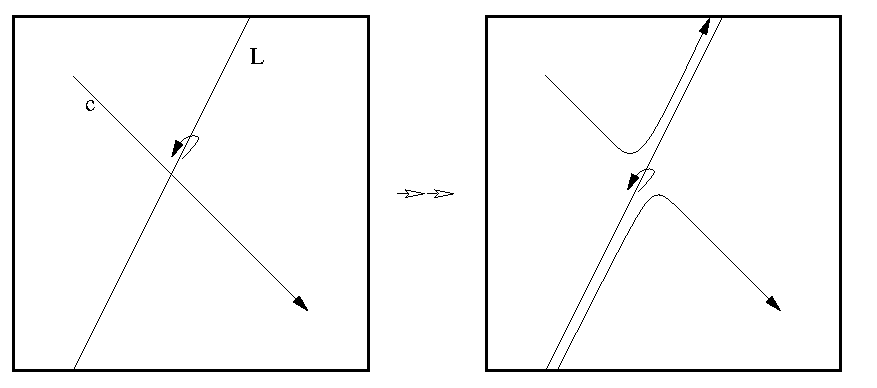
\includegraphics[width=0.85\linewidth]{figures/fig1.pdf}
  \caption{Dehn 扭转 $\tau_L$ 对测试曲线 $c$ 的作用。（原文 Figure 1，第 18 页）}
  \label{fig:dehn-twist}
\end{figure}

\subsection{分次辛几何}
\label{subsec:graded-sympl}

下面把上述想法推广，以纳入 "分次"。这些材料都可在 [18] 中找到。

先回忆：任何流形 $M$ 上都有自然的纤维丛 $\pi: \mathrm{Gr}(n,M)\to M$，其纤维为 $\mathrm{Gr}(n,T_xM)$。若 $M$ 是 $2n$ 维辛流形，则可取拉格朗日子空间构成的子丛 $\mathrm{LGr}(M)\subset\mathrm{Gr}(n,M)$，称为 $M$ 的\emph{拉格朗日 Grassmann 流形}。对任意拉格朗日子流形 $L\subset M$，存在自然截面 $s_L: L\to\mathrm{LGr}(M)$（由 $s_L(x)=T_xL$ 给出）。若 $\phi: M\to M$ 是辛同胚，则有覆盖 $\phi$ 的映射 $\phi_*: \mathrm{LGr}(M)\to\mathrm{LGr}(M)$，由 $\phi_*(x,L_x)=(\phi(x),D\phi L_x)$ 给出。对任意拉格朗日子流形 $L$，它满足 $\phi_* s_L = s_{\phi(L)}\phi|_L$。

回忆：对相当好的空间 $X$ 与阿贝尔群 $A$，$X$ 的 $A$-覆盖（即带有 $A$ 的连续、逐纤维传递且忠实作用的覆盖空间）由 $H^1(X,A)$ 分类。

\begin{definition*}
设 $(M,\omega)$ 是辛流形。$M$ 的 \emph{Maslov 覆盖}（Maslov cover）是指 $\mathrm{LGr}(M)$ 的一个 $\ZZ$-覆盖 $\cL$，具有如下性质：若 $c\in H^1(\mathrm{LGr}(M),\ZZ)$ 分类 $\cL$，$x\in M$，而 $i_x: \mathrm{LGr}(T_xM)\to\mathrm{LGr}(M)$ 表示纤维的包含，则
\[
  i_x^*(c) = s_{T_xM}.
\]
\end{definition*}

回忆 $s_{T_xM}$ 表示 $\mathrm{LGr}(T_xM)$ 的 Maslov 类，它是 $H^1(\mathrm{LGr}(T_xM),\ZZ)$ 的典范生成元。由于 $\pi_1(\mathrm{LGr}(T_xM))=\ZZ$，特别可知 $\cL$ 是 $M$ 上的纤维丛，其纤维是 $\mathrm{LGr}(T_xM)$ 的万有覆盖。可以证明：Maslov 覆盖存在当且仅当 $2c_1(M)=0$（其中 $c_1(M)$ 表示切丛的第一陈类）。事实上，取 $M$ 上相容的近复结构，记 $\Delta_M=\Delta(M,\omega,I):=\Lambda^n(TM,\CC)^{\otimes 2}$。则 $M$ 的 Maslov 覆盖与 $\Delta_M$ 的平凡化的同伦类一一对应（特别地，它们构成 $H^1(M,\ZZ)$ 上的仿射空间），见 [18, lemma 2.2] 及其前面的讨论。

% [Tutor Note: 这是全节最容易被跳过的论证，实质如下。$\Delta_M=\Lambda^n(TM,\mathbb C)^{\otimes 2}$ 是复线丛，其单位圆丛 $S(\Delta_M)\to M$ 是 $S^1$-丛，第一陈类为 $c_1(\Delta_M)=2c_1(M)$。而 Maslov 覆盖 $\cL$ 在每个纤维上正是 $\mathrm{LGr}(T_xM)$ 的万有覆盖，这等价于把 $S(\Delta_M)$ 的纤维方向 "展开" 成 $\mathbb R$；因此 $\cL$ 与 $S(\Delta_M)$ 的平凡化是同一件事。$S^1$-丛可平凡化 $\iff$ 其第一陈类为零，即 $2c_1(M)=0$；平凡化的同伦类构成 $H^1(M,\mathbb Z)$ 的仿射空间（两个平凡化的比是 $M\to S^1$ 的映射类）。]

% [Tutor Note: 定义中的条件 $i_x^*(c)=s_{T_xM}$ 必须盯紧：$c$ 是 $M$ 上 $\mathrm{LGr}(M)$ 的 $H^1$ 类，把它拉回到纤维 $i_x$ 上，必须恰好是纤维的典范生成元（而不是它的某个整数倍）。若写成 $i_x^*(c)=n\,s_{T_xM}$（$n\ne 1$），得到的就不是 Maslov 覆盖，$\mathbb Z$-分次会整体缩并，Floer 复形的次数会出错。]

给拉格朗日子流形分次的主要理由如下：设 $(L_1,t_1)$ 与 $(L_2,t_2)$ 是分次拉格朗日子流形，$x\in L_1\cap L_2$。在 $\cL_x$ 中取从 $t_1(x)$ 到 $t_2(x)$ 的道路 $\gamma$。由于 $\cL_x$ 是 $\mathrm{LGr}(T_xM)$ 的万有覆盖，该道路在同伦意义下唯一。因此
\[
  \mu_x(L_1,L_2) := \mu(\pi\gamma)
\]
（右端表示定理 \ref{thm:4.1} 中道路的 Maslov 指标）是良定义的，称为 $x$ 的 \emph{Maslov 指标}。

% [Tutor Note: 这里 $\pi$ 指万有覆盖投影 $\cL_x\to\mathrm{LGr}(T_xM)$。注意 $\cL_x$ 是 Maslov 覆盖在 $x$ 处的纤维，$t_i(x)$ 是该纤维中的点，其投影才是拉格朗日子空间 $T_xL_i$；于是 $\pi\gamma$ 是 $\mathrm{LGr}(T_xM)$ 中从 $T_xL_1$ 到 $T_xL_2$ 的道路，$\mu(\pi\gamma)$ 正是定理 \ref{thm:4.1} 的路径 Maslov 指标。这个整数就是交点 $x$ 的 $\mathbb Z$-次数，它可以是负数——这正是分次框架比 $\mathbb Z/2$ 框架强的地方。]

称辛流形 $(M,\omega)$ 连同一个 Maslov 覆盖 $\cL$ 的选择为\emph{分次流形}（graded manifold）。所谓\emph{分次拉格朗日子流形}（graded Lagrangian），是指拉格朗日子流形 $L$ 连同 $s_L$ 的提升 $t_L: L\to\cL$。所谓\emph{分次辛同胚} $\phi: (M,\omega_M,\cL_M)\to(N,\omega_N,\cL_N)$，是指辛同胚 $\phi: M\to N$，连同覆盖 $\phi_*: \mathrm{LGr}(M)\to\mathrm{LGr}(N)$ 的 $\ZZ$-等变提升 $\phi_*: \cL_M\to\cL_N$。

分次辛同胚可按自然方式复合，记 $\Sym^{gr}(M)$ 为 $M$ 的分次辛同胚群。其中有一个中心子群 $\{\mathbf 1[n]\mid n\in\ZZ\}\simeq\ZZ$，$\mathbf 1[n]$ 由 $\phi=\mathbf 1$、$\phi_*(x)=x+n$ 给出（用覆盖上的 $\ZZ$-作用）。对任意分次自同构 $\phi$，记 $\phi[n]:=\mathbf 1[n]\phi=\phi\mathbf 1[n]$。注意 $\Sym^{gr}(M)$ 自然地作用在分次拉格朗日子流形的集合上。若 $L$ 是分次拉格朗日子流形，则用 $L[n]$ 记分次拉格朗日子流形 $\mathbf 1[n](L)$。此外，若 $\phi_1$ 与 $\phi_2$ 由辛同伦连接，则 $\phi_1$ 的分次诱导 $\phi_2$ 的分次。

% [Tutor Note: 这里的 $\mathbb Z$-作用必须盯紧符号：$\mathbf 1[n]$ 把覆盖的纤维坐标加 $n$，而 $L[n]:=\mathbf 1[n](L)$ 使所有交点的次数整体减去 $n$，即 $\mu_x(L[n],L')=\mu_x(L,L')-n$。理由：把 $t_1(x)$ 换成 $t_1(x)+n$ 后，覆盖中从新起点到 $t_2(x)$ 的道路投影到 $\mathrm{LGr}$ 后与原来的道路相差一个环路，该环路的 Maslov 指标正是 $-n$。$[1]$ 就是 Floer 复形的平移函子；若这个符号取反，$m_1^2=0$ 与 $m_2$ 的 Koszul 符号都会错。又因为 $\mathbf 1[n]$ 是中心元，$\phi[n]=\mathbf 1[n]\phi=\phi\mathbf 1[n]$ 才无歧义。]

% [Tutor Note: "若 $\phi_1$ 与 $\phi_2$ 由辛同伦连接，则 $\phi_1$ 的分次诱导 $\phi_2$ 的分次" 的论证被省略了：$\phi$ 的分次是 $\phi_*:\mathrm{LGr}(M)\to\mathrm{LGr}(M)$ 的提升的同伦类；辛同伦给出 $\phi_{1*}$ 与 $\phi_{2*}$ 之间的同伦，而同伦的映射其提升之间存在典范对应。这也说明分次在 $\Sym^{gr}(M)$ 上只依赖于连通分支。]

可以用上同调描述哪些辛同胚与拉格朗日子流形可分级、以及有多少种分次，见 [18, lemmas 2.3 and 2.4]。我们不需要这些。

\subsubsection{更显式的描述}
\label{subsec:graded-explicit}

设 $(M,\omega)$ 是辛流形，取定相容近复结构。设有非零截面 $\Omega\in\Delta_M$，满足 $|\Omega|\equiv 1$（即 $\Delta$ 的一个平凡化）。令
\[
  \cL_\Omega = \mathrm{LGr}(M)\times_{s,\Delta,c}\RR = \{(L,r)\mid s(L)=c(r)\}.
\]
这里 $\RR$ 表示平凡丛，$c: \RR\to S(\Delta)$ 是由 $\Omega$ 诱导的自然覆盖，而 $s: \mathrm{LGr}(M)\to\Delta$ 是自然映射。这是一个 Maslov 覆盖；可以证明事实上所有 Maslov 覆盖都这样得到。

% [Tutor Note: 这一步的实质是两个 $\mathbb Z$-覆盖之差：任取 Maslov 覆盖 $\cL$，它与 $\cL_\Omega$ 的差别是一个沿纤维方向为常数的连续函数，因而来自 $M$ 上的映射 $M\to S^1$，即 $H^1(M,\mathbb Z)$ 中的一个类。这就同时给出 "所有 Maslov 覆盖都如此" 与 "$H^1(M,\mathbb Z)$-仿射结构" 两条结论。]

现设 $L$ 是 $M$ 的拉格朗日子流形，$t_L: L\to\cL_\Omega$ 是分次。则可写 $t_L(x)=(s(s_L(x)),\tilde s_L(x))$，其中 $\tilde s_L: L\to\RR$ 是某个函数。此时
\[
  e^{2\pi i\tilde s_L(x)}\Omega(x) = s(s_L(x)),
\]
而这样的（连续）函数与 $L$ 的分次一一对应。

类似地，若 $\phi: M\to M$ 是辛自同构，则给 $\phi$ 一个分次，等同于给一个连续函数 $\tilde s_\phi: \mathrm{LGr}(M)\to\RR$，使得对任意 $x\in M$ 与 $L\in\mathrm{LGr}(M)_x$ 有
\[
  s(D\phi(L)) = e^{2\pi i\tilde s_\phi(L)}\Omega(x).
\]

% [Tutor Note: 上式两边严格说应在同一点取值：$s(D\phi(L))$ 落在 $\Delta$ 的 $\phi(x)$ 纤维上，而右端写的是 $\Omega(x)$。按原文的约定（$\Omega$ 是整体平凡化，$|\Omega|\equiv1$ 故可用它把各纤维的相位统一到 $\mathbb C$），这种写法可以接受；但若改用 $x$ 与 $\phi(x)$ 不同处的 $\Omega$，$\tilde s_\phi$ 会多出 $\phi$ 的相位项。核对 [18] 时请注意这一约定。]

现设 $(\phi,\tilde s_\phi)$ 与 $(\psi,\tilde s_\psi)$ 是分次辛同胚，而 $(L,\tilde s_L)$ 是分次拉格朗日子流形。则容易验证
\begin{align*}
  \tilde s_{\psi\phi} &= \tilde s_\phi + \tilde s_\psi\circ D\phi,\\
  \tilde s_{\phi(L)} &= \tilde s_L\circ\phi^{-1} + \tilde s_\phi\circ s_L\circ\phi^{-1}.
\end{align*}

% [Tutor Note: 这两式是 "分次" 的复合律，符号极容易错。第一式：先做 $\phi$ 再做 $\psi$，相位要加上 $\tilde s_\psi$ 在 $D\phi$ 处的值（因为 $\psi$ 的相位是在切空间上评价的）。第二式右端的 $\phi^{-1}$ 出现两次，是因为左端 $\tilde s_{\phi(L)}$ 是定义在 $\phi(L)$ 上的函数；若把它看成定义在 $L$ 上的函数（即比较 $\tilde s_{\phi(L)}\circ\phi$），就得到 $\tilde s_L+\tilde s_\phi\circ s_L$ 这种更常见的写法。两种写法差一个拉回，不是笔误。]

\subsubsection{例：平坦环面}
\label{subsec:maslov}

现在考虑环面 $T=\CC/\ZZ^2$。它带有自然的（常值）辛形式与全纯结构。我们得到 $\Delta_T$ 的一个平凡化 $\Omega=\partial/\partial z^{\otimes 2}$。在同伦意义下，其余所有平凡化都有形式 $\Omega_{m,n}(x,y)=e^{2\pi i(mx+ny)}\Omega$。于是对 $m,n\in\ZZ$ 得到相应的 Maslov 覆盖 $\cL_{m,n}$；由上面的讨论，这给出了全部 Maslov 覆盖。

% [Tutor Note: 记号存疑：$\Delta_M$ 按定义是 $\Lambda^n(TM,\mathbb C)^{\otimes 2}$，即切丛的最高外幂的平方，而原文写的 $\Omega=\partial/\partial z^{\otimes 2}$ 用的是切向量（$\partial_z$）而非余切向量（$dz$）。在 Hermite 度量下二者可（共轭线性地）等同，故不一定是笔误；但与 [18] 对照时须统一约定，否则 $s(L)$ 与 $e^{2\pi i\tilde s}\Omega$ 的相对相位会差一个共轭。另注意这里的 $z$ 是复坐标，$x,y$ 是 $T$ 上的实坐标，$\Omega_{m,n}$ 的相位因子 $e^{2\pi i(mx+ny)}$ 正是 $H^1(T,\mathbb Z)$ 的仿射参数。]

现在容易验证：相对于与全纯平凡化 $\Omega$ 对应的覆盖 $\cL=\cL_{0,0}$，一个拉格朗日圆周可分级当且仅当它不是可缩的。相反，若 $(m,n)\ne(0,0)$，则可缩圆周仍然不可分级，但此时总还存在进一步的（非可缩的）不可分级圆周。因此全纯平凡化是 Maslov 覆盖的一个自然选择。此外，对这个 Maslov 覆盖的选取，$T$ 的任意辛自同构都可分级。（所有这些陈述都是容易的练习。）

% [Tutor Note: "easily checked" 的实际内容是三步：(i) 可分级 $\iff$ $s_L$ 可提升到 $\cL$ $\iff$ 沿 $L$ 绕一周 Maslov 指标的变化为零（即 $s_L^*(c)=0\in H^1(L,\mathbb Z)$）；(ii) 对 $\mathbb C/\mathbb Z^2$ 与全纯平凡化逐同调类计算该指标，得到 "可缩圆周不可分级、非可缩圆周可分级"；(iii) 换用 $\cL_{m,n}$ 后，$c$ 类被乘以相位 $e^{2\pi i(mx+ny)}$，可分级圆周的集合随之改变，并且总有额外的非可缩不可分级圆周出现。这条练习的关键结论是：Maslov 覆盖的选择会改变 A-模型的分次数据，故镜像对称的陈述必须先固定它。]

% [Tutor Note: 为什么全纯平凡化是 "自然" 的？因为它由 $T$ 的复结构直接给出，因而与 B-模型侧的代数结构（$\mathcal O_T$ 与全纯坐标）典范相容；HMS 中的分次对应正是在这一选择下才逐次相符。换成 $\cL_{m,n}$ 相当于对 A-模型作一次 "平坦的 $\mathbb Z$-平移 twisting"，物理上对应一个不改变拓扑、但改变分次数据的背景场。]

\subsection{辛曲面的 Fukaya 范畴}
\label{subsec:fuk-surface}

下面描述紧辛曲面（带 Maslov 覆盖的选择）的 Fukaya 范畴，即环面 $T$（带某种辛形式与 Maslov 覆盖的选择）。密切相关的讨论见 [1]，也见我们的主要参考 [19]。

% [Tutor Note: 原文此处脱字："the Fukaya category a compact symplectic surface" 应为 "the Fukaya category of a compact symplectic surface"，译文按文意补出 "的"。]

设 $L_1,L_2,\dots,L_n$ 是 $T$ 中的分次拉格朗日圆周（即紧连通拉格朗日子空间，并带分次的选择），且两两横截。则对 $i\ne j$，集合 $L_i\cap L_j$ 有限。用 $\Lambda_t$ 记形式幂级数 $\sum_{n>0}a_n t^{b_n}$ 的域，其中系数 $a_n\in\CC$，实指数 $b_n\in\RR$ 当 $n\to\infty$ 时趋于无穷。于是构成 \emph{Floer 链空间}
\[
  CF^*(L_i,L_j) = \bigoplus_{x\in L_i\cap L_j} [x]\Lambda_t,
\]
其中 $[x]$ 是次数为 $\mu_x(L_i,L_j)$ 的形式生成元。

% [Tutor Note: 系数域必须用实指数的形式幂级数 $\Lambda_t$（Novikov 域），而不是普通多项式：多边形计数一般有无穷多个（面积可以趋于无穷），$A_\infty$ 关系中每个系数都是无穷和，需要一个既允许无穷和、又保持 "最低次项"（按面积过滤）有限的系数域。实指数 $b_n\to\infty$ 保证在任一有界面积区间内只有有限项，这是 Gromov 紧性在代数侧的对应物。]

下面说明如何定义运算
\[
  m_n : CF^*(L_n,L_{n-1})\otimes\cdots\otimes CF^*(L_1,L_2) \longrightarrow CF^*(L_1,L_n),
\]
使得只要 $A_\infty$-关系有意义就成立。具体地，令
\[
  m_n(p_{n-1},\dots,p_1) = \sum_{q\in L_1\cap L_n} C(q;p_1,\dots,p_{n-1})[q].
\]
这里 $p_i\in L_i\cap L_{i+1}$。下面解释如何计算系数 $C(q;p_1,\dots,p_{n-1})$。

% [Tutor Note: 原文疑误：$m_n$ 的定义域写成 $CF^*(L_n,L_{n-1})\otimes\cdots\otimes CF^*(L_1,L_2)$，但按紧接着的 $p_i\in L_i\cap L_{i+1}$ 以及定理 \ref{thm:4.2} 第 (1) 条（$\Hom(L_{n-1},L_n)\otimes\cdots\otimes\Hom(L_1,L_2)\to\Hom(L_1,L_n)$），第一个因子应为 $CF^*(L_{n-1},L_n)$。两处不自洽，译文保留原文定义式，实际计算以定理 \ref{thm:4.2} 的写法为准。]

用 $D_n$ 记单位圆盘，其边界上依次有标号点 $P_1,P_2,\dots,P_{n-1}$ 与 $Q$（按此顺序）。用 $\gamma_i$ 记终止于 $P_i$ 的边界弧段。用 $\mathcal{M}(q;p_1,\dots,p_{n-1})$ 记浸入多边形 $u: D_n\to X$ 的等价类集合，满足：(1) $u$ 保定向，且在 $P_i$ 与 $Q$ 之外是嵌入；(2) $u$ 在 $P_i$ 与 $Q$ 处有凸角；(3) $u(P_i)=p_i$ 且 $u(Q)=q$；(4) $u(\gamma_i)\subset L_i$。两个嵌入多边形若相差 $D_n$ 的一个微分同胚，则视为等价。

% [Tutor Note: 原文疑误：此处写 $u:D_n\to X$，但本节只讨论环面 $T$，前面的记号也一直用 $T$，应为 $u:D_n\to T$。译文保留原文的 $X$ 以便对照。]

然后令
\[
  C(q;p_1,\dots,p_{n-1}) = \sum_{u\in\mathcal{M}(q;p_1,\dots,p_{n-1})} \pm\, t^{\int_{D_n} u^*\omega}.
\]
这里 $\pm$ 表示一个我们不打算解释的符号\footnote{我们不需要这个符号，只需要存在某种符号规则使下面的定理成立。}。

% [Tutor Note: 脚注 "只需要存在符号规则" 是轻描淡写：一般情形下符号来自拉格朗日的相对 spin（或 Pin）结构与定向数据，且必须精密到使 $m_1^2=0$ 与 $A_\infty$ 结合律成立；在二维情形这些都可显式选出。原文略去符号不影响定理 \ref{thm:4.2} 的陈述，但若要真正算 $m_2$ 的显式公式（§6 的计数），符号约定必须与 [19] 对齐，否则 $A_\infty$ 关系的验证会差号。]

遗憾的是，这里没有篇幅解释为什么这样得到满足 $A_\infty$-关系的映射。下面的定理汇总了我们将要用到的 Fukaya 范畴的性质。

\begin{theorem}\label{thm:4.2}
设 $(T,\omega,\cL)$ 是分次流形，其中 $T$ 是环面。\emph{Fukaya 范畴} $\Fuk(T)$ 以分次拉格朗日子流形 $(L,t_L)$ 为对象。此外：
\begin{enumerate}[leftmargin=1.8em, itemsep=2pt, topsep=2pt]
  \item 若 $L_1,L_2\in\Fuk(T)$ 横截，则 $\Hom_{\Fuk(T)}(L_1,L_2)=CF^*(L_1,L_2)$。若 $L_1,\dots,L_n$ 横截，则
  \[
    m_n^{\Fuk(T)}: \Hom(L_{n-1},L_n)\otimes\cdots\otimes\Hom(L_1,L_2) \longrightarrow \Hom(L_1,L_n)
  \]
  就是上面构造的映射。
  \item 存在 $\Sym^{gr}(T)$ 在 $\Fuk(T)$ 上的作用。在对象上，它就是先前构造的作用。此外，若 $\phi$ 是哈密顿同伦于恒等的分次辛同胚，则它在 $\Fuk(T)$ 上的作用拟同构于恒等函子。
  \item 若 $L$ 是拉格朗日圆周，$\tilde\tau_L$ 表示 $L$ 上带标准分次的辛 Dehn 扭转（symplectic Dehn twist），而 $L'\in\Fuk(T)$，则
  \[
    T_L(L') \simeq \tilde\tau_L(L').
  \]
  这里 $T_L$ 表示第 \ref{subsec:ainf-twisting} 节中的代数扭变函子（twist functor）。
\end{enumerate}
\end{theorem}

% [Tutor Note: 第 (2) 条里 "拟同构于恒等函子" 不能加强为 "等于"：哈密顿同伦只保证作用在对象上同构、在态射上差一个同伦，且这个同构本身依赖同伦的选取；这正是 A-模型侧 "规范等价" 的含义。与第 (3) 条合起来看，$\Sym^{gr}(T)$ 的作用把几何的自同构变成范畴的自等价，而哈密顿同伦类对应的是 "平凡" 的那部分。]

% [Tutor Note: 第 (3) 条是本文的核心对应之一：代数侧沿球状对象 $L$ 的扭变函子 $T_L$（在导出范畴中的标准公式是 "evaluation 的锥"）与辛侧沿 $L$ 的 Dehn 扭转 $\tilde\tau_L$ 在对象上一致。几何图像：Dehn 扭转把穿过 $L$ 的测试曲线 $c$ 在一侧剪开再粘回（图 \ref{fig:dehn-twist}），对交点计数的效果等同于把 $c$ 卷过 $L$；$T_L$ 的锥公式正是这一操作的代数化。注意必须用带 "标准分次" 的 $\tilde\tau_L$：否则 $\mathbb Z$-次数会错位，$\tilde\tau_L(L')$ 与 $T_L(L')$ 只能同构到某个平移 $[n]$ 为止，定理就不成立。]
